\chapter{Conversione del modello}

\section{Spiegazione rapida del modello originale}

Gu

\section{PyTorch e PyTorch Mobile}

PyTorch è uno dei due framework di machine learning più popolari.
Esso è sviluppato da Facebook (ora Meta), ed è basato su Python.

Il workflow del framework si può riassumere in questo modo:

\begin{itemize}
    \item Caricare i dati di training e test, come \texttt{Dataset}, 
    incapsulati poi dentro ad un \texttt{Dataloader} per permettere l'iterazione.
    \item Creazione di un modello, definendo i vari layer della rete neurale usando
    delle funzioni incorporate nel framework, dentro ad una classe \texttt{nn.Module}.
    \item Training, ripetendo delle iterazioni sul dataloader nelle quali si computa
    l'errore di predizione, e in base a esso si calcolano i nuovi pesi, per poi verificare
    il miglioramento dell'accuratezza tramite il dataset di test.
    \item Uso dei modelli così allenati caricando i pesi e usando la stessa classe Module
    creata in precedenza, in modalità \emph{no\_grad} per differenziare dallo stato di
    training (impedendo così la modifica dei pesi), e ottenendo così delle predizioni.
\end{itemize}

PyTorch normalmente gestisce dati in forma di tensori, e offre funzioni di libreria per
convertire tipi di dato comune da e a tensori, in particolare, per lo scopo di questo
progetto, permette di convertire immagini in tensori e vice versa.

\subsection{PyTorch Mobile}

PyTorch Mobile è un runtime per PyTorch su dispositivi mobile e embedded, al momento in
beta. Supporta i sistemi operativi iOS, Android, e Linux, offrendo API per le operazioni
di uso comune necessarie a integrare le reti neurali in questo genere di applicazioni,
oltre a supportare operazioni di ottimizzazione come la quantizzazione. Offre anche 
un interprete ottimizzato per PyTorch su Android e iOS, che compila selettivamente solo
le componenti del framework necessarie all'app.

Si può anche sfruttare TorchScript per migliorare e facilitare l'ottimizzazione di modelli
a dispositivi mobile. TorchScript è un linguaggio creato ad hoc per PyTorch, ed è una 
sottoparte del linguaggio Python, in particolare delle parti necessarie a rappresentare reti 
neurali. Inoltre, TorchScript ha tipi delle variabili statici, a differenza di Python.

PyTorch offre funzioni per compilare codice Python in TorchScript, sottostando a certi
vincoli. Per esempio, \texttt{torch.jit.script} permette di trasformare \texttt{Module}
o funzioni in \texttt{ScriptModule} e \texttt{ScriptFunction}, delle copie dell'originale
convertite in TorchScript, che poi potranno essere salvati tramite \texttt{torch.jit.save}
su file. In particolare, gli \texttt{ScriptModule} avranno gli stessi parametri del modello
originale, che verranno salvati su file insieme al modello, permettendo quindi di caricare
successivamente sia la logica che i parametri allenati del modello dallo stesso file.

PyTorch Mobile sfrutta TorschScript per permettere di caricare il modello sul framework 
e nel linguaggio di destinazione (per esempio, Java o Kotlin per Android). Questo permette
di creare il modello usando l'API di PyTorch in Python, senza dover "ricreare" il codice
Python del modello originale in Java o altri linguaggi. Di conseguenza, l'API di PyTorch 
Mobile per Android è molto minimale, offrendo funzioni per caricare modelli di TorchScript, 
wrapper per tensori e modelli, e un wrapper generico ai tipi di TorschScript, \texttt{IValue}.

L'API non offre funzioni equivalenti alla maggior parte dei metodi di libreria PyTorch, 
supponendo che l'utente usi direttamente le funzioni in Python e le carichi nell'applicazione
convertite in formato TorschScript; l'API Mobile è quindi generalmente disaccoppiata dalla
libreria di Pytorch.

Il workflow generale per convertire modelli a PyTorch Mobile è descritto nella figura 
\ref{fig:workflow_pytorch_mobile}. Una volta ottenuto il modello convertito, e trasformati
i dati in \texttt{IValue} tensori nell'API del sistema di destinazione, si chiama il metodo
\texttt{forward} del modello convertito per ottenere la propria predizione.

Una nota importante è il diverso formato dei modelli TorchScript ottimizzati per mobile: 
essi vengono salvati tramite la funzione interna alla classe \texttt{ScriptModule}
\emph{\_save\_for\_lite\_interpreter}, in un formato diverso rispetto a quelli salvati tramite
\texttt{torch.jit.script}, come si evince dall'estensione suggerita dalla documentaizone .ptl
invece di .pt. Nella versione attuale di PyTorch Mobile, esistono due versioni diverse della
libreria (per Android, \emph{org.pytorch.pytorch\_android} e 
\emph{org.pytorch.pytorch\_android\_lite}): ogni versione è in grado di caricare solo i file
TorchScript salvati dalla funzione corrispondente, e non l'altra; questo al momento offre
problemi per la conversione di funzioni convertite a \texttt{ScriptFunction}, che attualmente
non dispone di un metodo \emph{\_save\_for\_lite\_interpreter}, impedendo quindi di caricare 
funzioni convertite a TorchScript in un contesto \emph{lite}. Quindi, l'unico modo di usare
le varie funzioni di libreria di PyTorch all'interno di applicazioni mobile, nella versione 
attuale, è usarle all'interno di un \texttt{Module} di rete neurale.

\begin{figure}[!bh]
    \centering
    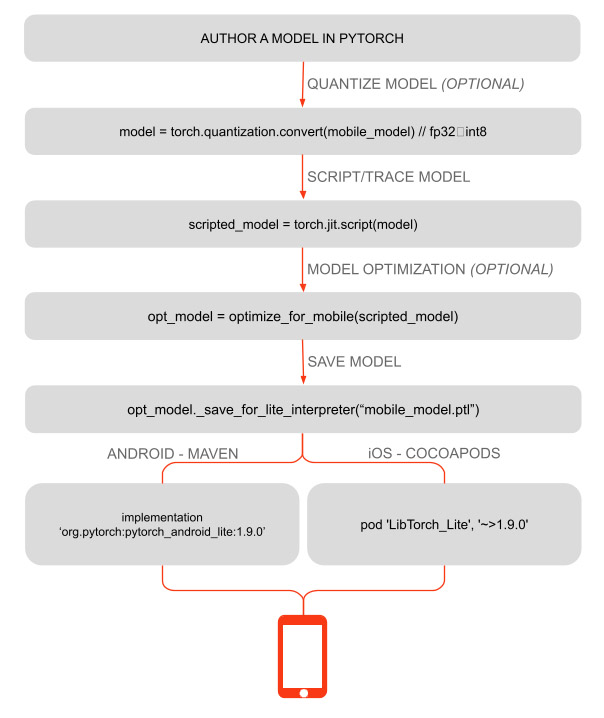
\includegraphics[width=0.7\textwidth]{img/pytorch_mobile_workflow.jpg}
    \caption{Fonte dell'immagine: https://pytorch.org/mobile/home/}
    \label{fig:workflow_pytorch_mobile}
\end{figure}

\FloatBarrier

\subsection{Compensazione di lacune nell'API Mobile}

Come detto sopra, l'API di PyTorch Mobile, almeno su Android, è molto essenziale, assumendo
che l'utente farà il grosso della logica del modello in Python tramite PyTorch, per poi
convertirlo in TorchScript e caricarlo. Mancano quindi i vari metodi per manipolare tensori,
e gestire i set di dati, e nella versione attuale di PyTorch Mobile, come sopra, non è possibile
caricare funzioni TorschScript in un contesto di PyTorch Mobile lite. Nel caso in cui servano 
nell'applicazione funzionalità della libreria PyTorch all'esterno di un modello, sarà necessario
reimplementarle.

\subsubsection*{Dataset}

In questo progetto è stato scelto di reimplementare la classe Pytorch Dataset, 
nel caso specifico di interesse al progetto, vale a dire un set di immagini rappresentanti
fotogrammi di un video, da caricare a due a due in ogni iterazione per interpolare i fotogrammi
tra esse. Questo permette di riprodurre il comportamento dell'implementazione originale di
SuperSlowMo in Python, usando un codice molto simile.

È stata quindi creata una classe \texttt{VideoDataset}, che implementa un'interfaccia 
\texttt{IDataset}, definite in maniera sintetica in seguito:

\begin{lstlisting}
public interface IDataset<T> extends Iterable<T> {
    public abstract T get(int index);
    public abstract int len();
}

public class VideoDataset<T> extends Dataset<Pair<T, T>> {
    private IImageLoader imageLoader;
    private String root;
    private String[] framePaths;
    private Function<Bitmap, T> transform;
    private Size origDim;
    private Size dim;

    public static <T> VideoDataset<T> withRootPath(String root, 
        Function<Bitmap, T> transform) {...}
    public static <T> VideoDataset<T> withContextAssets(Context context, 
        String root, Function<Bitmap, T> transform) {...}

    [...]
}
\end{lstlisting}

VideoDataset viene creata a partire da set di immagini (specificati o fornendo una cartella
nel file system Android, oppure una cartella negli asset dell'applicazione), e permette di 
fornire una funzione Transform che funziona in modo analogo all'argomento \emph{transform}
della classe \texttt{Dataset} di PyTorch: se presente, viene applicata su ogni immagine
durante l'iterazione del dataset, trasformandola in un tipo di dato diverso prima 
dell'elaborazione. 

Un uso comune di questa funzionalità è convertire immagini (classe
\texttt{Bitmap} in Android) in tensori, quindi \texttt{IValue} di tipo Tensore nell'API
PyTorch Mobile; l'API offre una funzione per questa conversione, 
\texttt{TensorImageUtils.bitmapToFloat32Tensor}. Un esempio di uso con \texttt{VideoDataset} 
è il seguente:

\begin{lstlisting}
videoFrames = VideoDataset.withRootPath(
    framesDir, 
    bitmap -> TensorImageUtils.bitmapToFloat32Tensor(bitmap,
        TensorImageUtils.TORCHVISION_NORM_MEAN_RGB,
        TensorImageUtils.TORCHVISION_NORM_STD_RGB
    )
);
\end{lstlisting}

\subsubsection*{Concatenazione Tensori}

Mancando le funzioni di PyTorch per svolgere operazioni tra Tensori, in particolare
\texttt{torch.cat}, in una prima versione del progetto era stato necessario reimplementare
questa funzione in Java. Non viene riportato il codice data la lunghezza, dovendo gestire 
separatamente i diversi casi di tipi primitivi contenuti dentro al tensore a causa della rigida
gestione degli array da parte di Java.

Nelle versioni successive del progetto, è stato possibile spostare tutto il codice che
necessitava di operazioni su tensori dentro al modello convertito in TorschScript, evitando
la necessità di reimplementare questa funzione.

\subsubsection*{Conversione da Tensori a Bitmap}

Come sopra, PyTorch Mobile offre una funzione per convertire immagini, quindi la classe
\texttt{Bitmap} nell'API Android, vale a dire \texttt{TensorImageUtils.bitmapToFloat32Tensor},
e alcune funzioni analoghe per altri tipi di dato del tensore. Notevolmente, nella versione 
attuale al momento dello sviluppo di questo progetto manca una funzione per la conversione
nella direzione opposta, vale a dire da tensore a immagine, cosa necessaria per reti neurali
che producono immagini come output, come questa.

È stato quindi necessario riprodurre questa funzionalità:

\begin{lstlisting}
public static Bitmap bitmapFromRGBImageAsFloatArray(float[] data, 
    int width, int height) {...}
\end{lstlisting}

Una prima versione portava a gravi artefatti nella conversione dello spazio RGB, che 
distorcevano le aree più luminose dell'immagine; la seconda versione, quella attuale, 
tiene conto della media e della deviazione standard dello spazio RGB di interesse in fase di
conversione, usando i valori forniti dall'API PyTorch Mobile, 
\texttt{TORCHVISION\_NORM\_MEAN\_RGB} e \texttt{TORCHVISION\_NORM\_STD\_RGB}. Un esempio di 
questo artefatto è in figura \ref{fig:img_conversion_error}.

\begin{figure}[!bh]
    \centering
    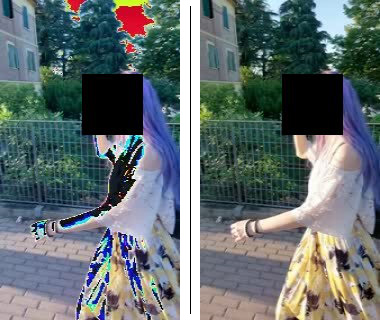
\includegraphics[width=0.85\textwidth]{img/conversione_img_errore.jpg}
    \caption{Errore nella conversione tensore $\rightarrow$ bitmap. A sinistra la prima versione, 
    a destra la versione corretta. Si noti la distorsione nelle aree luminose e le leggere
    differenze nella temperatura del colore.}
    \label{fig:img_conversion_error}
\end{figure}


\FloatBarrier

\section{Adattamento del modello a Pytorch Mobile}
Fillo

\subsection{Limiti}




FONTI

https://pytorch.org/javadoc/1.9.0/

https://pytorch.org/mobile/home/